%
% Hauptdatei
%


\documentclass[pdftex,a4paper,11pt,DIV15,BCOR20mm,parskip,numbers=noenddot]{scrbook}

	\usepackage{german, ngerman} %Deutsche Trennungen, Anf�hrungsstriche und mehr
	\usepackage[ngerman,german]{babel} % dt. Sprache laden (u.a. auch Ausgabe feststehender Begriffe in deutsch wie etwa Inhaltsverzeichnis statt table of contents)
	\usepackage[latin1]{inputenc} % Zeichenkodierung laden f�r Unix/Windows-Systeme
	\usepackage[babel,german=quotes]{csquotes} % Deutsche Eingabe von �,�,�,� erlauben	
	\usepackage[T1]{fontenc}
  \usepackage[pdftex]{color} 
  \usepackage{setspace} % Das Paket setspace erm�glicht ein einfaches Umstellen von normalem, anderthalbfachen oder doppeltem Zeilenabstand.
  \usepackage{graphics} %Zum Einbinden von Grafiken
  \usepackage[pdftex]{graphicx}  
	\usepackage[final]{listings}  % erm�glicht die Darstellung von (Programm-)Quellcode in der Arbeit
  \usepackage{ae,aecompl}  % ben�tigt zur PDF-Erzeugung, vgl http://dsanta.users.ch/resources/type1.html
  \usepackage[normalem]{ulem} % erm�glicht das Unterstreichen von Text
  \usepackage{amsfonts} % ok-zeichen usw
  \usepackage{scrpage2}
  \usepackage{bibgerm}
  \usepackage{array} % f�r tabellen

	% Beliebige Farben definieren (bei Bedarf auskommentieren und selbst benennen und festlegen)
%	\definecolor{hellblau}{RGB}{238,242,247}
	
	\usepackage{colortbl} % f�r farbige Tabellen
	\usepackage{longtable} % f�r mehrseitige Tabellen
%	\usepackage{booktabs} % f�r tabellen: baut \midrule, \toprule und \bottomrule ein
%	\setlength{\tabcolsep}{30pt} % in Tabellen: Padding des Spalten nach links und rechts
	\renewcommand{\arraystretch}{1.25} % in Tabellen: Padding des Textes nach oben und unten in Prozent

	% Benutzt man bestimmte Spaltendefinitionen (hier: Spaltentyp p mit 25% Breite) �fter, kann man diese hier auslagern und unter einem bestimmten Buchstaben (hier: A) speichern
%	\newcolumntype{A}{p{0.25\textwidth}} 

	\usepackage{nomencl} % Package f�r ein Abk�rzungsverzeichnis
	\renewcommand{\nomname}{Abk�rzungsverzeichnis} % Deutsche �berschrift
	\setlength{\nomlabelwidth}{.20\hsize} % Breite eines Eintrags
	\renewcommand{\nomlabel}[1]{#1 \dotfill} % Auff�llen mit Punkten
	\setlength{\nomitemsep}{-2\parsep} % Zeilenabstand verkleinern
	\makenomenclature  % Datenbank des Abk�rzungsverzeichnisses beim Kompilieren des Textes erzeugen

	% fuer Literaturverweise
	\usepackage[numbers,square]{natbib}
	\bibpunct{[}{]}{;}{a}{}{;} % Natbib konfigurieren, so da� im text [M�ller 2006] erscheint und keine runden Klammern o.�.
	\renewcommand{\cite}{\citep} % \cite zu \citep umwandeln, so dass im Text \cite{Mueller.2006} f�r Referenzen verwendet werden kann.
%	\usepackage{url} % damit im LitVZ auch so etwas wie 'M�ller 2006: Vortrag zum Thema XY (Powerpoint-Pr�sentation)' steht; (Dateiendungen werden also textuell repr�sentiert)

	%% Verhindert, dass im Literaturverzeichnis nach der Nennung von [Mueller 2006] die Seite umgebrochen wird und die Autoren + Buchtitel etc. auf der n�chsten Seite landen
	%% Es wurde daher \noparagraphbreak in der natdin.bst bei der Ausgabe der Elemente erg�nzt
	%% siehe http://groups.google.de/group/de.comp.text.tex/browse_thread/thread/9ca4c681e2063fbd/f7eb3eec044b058e
	\makeatletter
	\def\noparagraphbreak{\interlinepenalty10000
	  \@itempenalty-\@highpenalty}
	\makeatother 


	% Fu�noten werden im gesamten Dokument fortlaufend hochgez�hlt und nicht nur kapitelweise, vgl. http://www.golatex.de/nummerierung-der-fussnoten-durchgehend-im-gesamten-dokument-t2042.html
	\usepackage{chngcntr}
	\counterwithout{footnote}{chapter}

	\setlength{\emergencystretch}{1em} % F�r den Fall, dass Zeilen im 1. Anlauf nicht richtig umgebrochen werden k�nnen, einen 'Notfallraum' einrichten (vgl. http://www.golatex.de/overfull-boxes-in-latex-t1979.html) 

	% Definitionen werden mit Hilfe von 'dfn' eingeleitet und k�nnen somit zentral formatiert werden.
	\newtheorem{dfn}{Definition}
	
	% entnommen aus http://www.siart.de/typografie/latextipps.xhtml#floats
	\renewcommand{\floatpagefraction}{0.8} % gibt den Bruchteil einer Seite, die f�r Gleitobjekte benutzt wird, an, der erreicht werden muss, bevor eine neue Seite angefangen wird. (Standard: 0.5; d.h. wenn ein Bild 51% der Seite einnimmt, wird extra f�r dieses Bild eine ganze Seite reserviert --> unsch�n)
	\renewcommand{\topfraction}      {0.8}
	\renewcommand{\bottomfraction}   {0.5} % \topfraction / \bottomfraction, gibt den Bruchteil einer Seite an, bis zu dem Gleitobjekte oben bzw. unten angeordnet werden sollen.
	\renewcommand{\textfraction}     {0.15} % gibt den Bruchteil einer Seite an, der mit Text belegt werden k�nnen muss.
	\makeatletter
	  \setlength{\@fptop}{0pt} % Wenn ein Float-Objekt allein auf einer Seite steht, soll es am oberen Rand der Seite erscheinen und nicht vertikal zentriert
	\makeatother
	
	% schrift auf palatino umstellen
  \usepackage{palatino}
  \setkomafont{sectioning}{\normalcolor\bfseries}


	% PDF-Support einbinden und konfigurieren
  \usepackage[
  	pdfstartview={Fit},   
  	pdffitwindow=true,
  	colorlinks,
  	linkcolor=black,
  	anchorcolor=black,
  	citecolor=black,
  	urlcolor=black
  ]{hyperref}
  \hypersetup
  {
  	pdftitle     = {Diplomarbeit zum Thema Sprachverarbeitung mit fokusierung auf Vocaltrennung mit hilfe eines LSTM-Netzes},
  	pdfsubject   = {Universit�t Hamburg / Department Informatik / ITG / Bachlorarbeit},
  	pdfauthor    = {Wajid Ghafoor},
  	pdfkeywords  = {Bachlorarbeit, Universit�t Hamburg}, % Hier kann eine beliebige Liste von Schl�sselw�rtern eingegeben werden, die z.B. Windows zur Indexierung/Suche benutzt
  	plainpages   = false 
  }
 
   
  % Zeilenabstand
  \setstretch{1.24}   

	% Strafpunkte, die beim Seitenumbruch vergeben werden, falls die erste Zeile eines Absatzes allein auf der vorangehenden Seite verbleibt. vgl http://www.jr-x.de/publikationen/latex/tipps/zeilenumbruch.html
	\clubpenalty=150

	% Strafpunkte, die beim Seitenumbruch vergeben werden, falls die letzte Zeile gerade noch auf die n�chste Seite umgebrochen wird. vgl http://www.jr-x.de/publikationen/latex/tipps/zeilenumbruch.html
	\widowpenalty=150  

  % Pagestyle definieren (nach Martins Template)
	\defpagestyle{diplHeadings}
	{ % es folgt: Definition des Seitenkopfes: 
	  % obere Linie
		(0pt,0pt)
		% linke Seite
		{\upshape \rlap{\pagemark} \hfill \headmark \hfill} % auf einer linken Seite soll LINKS die Seitenzahl stehen und mittig die Headline (headmark)
		% rechte Seite
		{\upshape \hfill \headmark \hfill \llap{\pagemark}} % auf einer rechten Seite soll RECHTS die Seitenzahl stehen und mittig die Headline (headmark)
		% falls Layout "one page"
		{}
		% untere Line
		(\textwidth,1pt)
	}
	{ % es folgt: Definition des Seitenfu�es: Wir wollen lediglich eine schwarze, �ber die komplette Seite gehende Linie erzeugen
	  % obere Linie
		(\textwidth,1pt)
		% linke Seite
		{}
		% rechte Seite
		{}
		% falls Layout "one page"
		{}
		% untere Linie
		(0pt,0pt)
	}  
	% Pagestyle auch f�r Chapter-Anfang einrichten
	\renewcommand*{\chapterpagestyle}{diplHeadings}
	\renewcommand*{\chapterheadstartvskip}{\vspace*{-\topskip}}
	\automark[section]{chapter}


	% R�nder	
	\setlength{\textwidth}{15cm}        % Textbreite
	\setlength{\textheight}{24cm}       % Texth�he
	\setlength{\topmargin}{-12mm}       % oberer Rand
  
 
  % Listingsformatierung (Quelltexte)
  \definecolor{lightgrey}{rgb}{0.90,0.90,0.90}
  \lstloadlanguages{XML}
  \lstset{
    tabsize=2,
    escapeinside={(*@}{@*)},
    captionpos=t,
    framerule=0pt,
    backgroundcolor=\color{lightgrey},
    basicstyle=\small\ttfamily,
    keywordstyle=\small\bfseries,
    numbers=left,
    fontadjust
  }    
%
% EOF
%  % Einbinden der Konfigurationen

\begin{document}


%
% Titelseiten Datei
%

\begin{titlepage}

	% Fehler "destination with the same identifier" unterdr�cken...
  \setcounter{page}{-1}

	% Titelseite
	\begin{figure}[h]
		\begin{minipage}[b]{25mm}
			
\includegraphics[width=25mm,clip]{images/logo_uhh}
		\end{minipage}
		\begin{minipage}[b]{2mm}
			
\includegraphics[width=1mm,height=24mm]{images/greypixel}
		\end{minipage}
		\begin{minipage}[b]{12 cm}
			{\sffamily
				{\Large Universit�t Hamburg } \\
				Fakult�t f�r Mathematik,\\
				Informatik und Naturwissenschaften \\
				Department Informatik \\
			}
		\end{minipage}
	\end{figure}

	\vfill
	
	\begin{center}
		% Diplomarbeit 
		\noindent { \huge
			Bachlorarbeit \\
					}
		\vspace{14mm}
		% Titel
		\noindent \textbf{\Large
		  <Sprachverarbeitung mit fokussierung auf vocaltrennung \\
		  mit Hilfe eines LSTM Netzes> \\		  
		}
		\vspace{10mm}
		
		\noindent {\large
		(Option:) In Kooperation mit:
		
		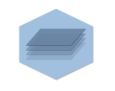
\includegraphics{images/logoitg.png}\\ %Firmenlogo
		<Firma> \\
		<Bereich / Abteilung>
		}
	\end{center}
	
	\vfill
	
	\noindent \textbf{<Wajid> <Ghafoor>} \\
	\noindent \rule{\textwidth}{0.4mm} 
	\noindent{\textrm{<3ghafoor@informatik.uni-hamburg.de>}} \\
	\noindent{\textrm{Studiengang <Informatik>}} \\
	\noindent{\textrm{Matr.-Nr. <6533381>}} \\
	\noindent{\textrm{Fachsemester <9>}} \\
	\begin{tabbing}
	\hspace{20em} \=  \kill
	Erstgutachter Universit�t Hamburg: \> Prof. Dr. Chris Biermann \\
	Zweitgutachter Universit�t Hamburg: \> <PhD Benjamin Milde> \\
		
	\hspace{20em} \=  \kill
	
	(Option)Betreuer <Firma>: \> <Vorname> <Name> \\
			
	\end{tabbing}
	
	% R�ckseite der Titelseite mit Zitat
	\newpage 
	\thispagestyle{empty}
	\setcounter{page}{0}

	% wenn man Lust auf ein Zitat hat...
	% ... ansonsten auskommentieren
	~\\ \vfill \noindent 
%	A distributed system is one where the failure of some \\
%	computer I've never heard of can keep me from getting my work done. \\
%	\textit{-- Leslie Lamport}
\end{titlepage}

%
% EOF
%



% pagestyle umschalten
\pagestyle{diplHeadings}

\nomenclature{IT}{Informationstechnik}
\nomenclature{WWW}{World Wide Web} % Einbinden der zentralen Datei, die alle Abk�rzungen enth�lt
%
% Inhaltsverzeichnis
%

% --> Seitennummerierung r�misch
\pagenumbering{Roman}
\setcounter{page}{1}
\pdfbookmark[1]{Inhaltsverzeichnis}{toc}

\tableofcontents
\cleardoublepage

%
% Abbildungs- und Tabellenverzeichnis
%
\listoffigures
\listoftables
\cleardoublepage

%
% Abk�rzungsverzeichnis ausgeben
%
\markboth{Abk�rzungsverzeichnis}{Abk�rzungsverzeichnis} % Kopfzeile anpassen, vgl. http://www.golatex.de/falsche-kopfzeile-im-abkuerzungsverzeichnis-t2074.html
\printnomenclature % Abk�rzungsverzeichnis
\cleardoublepage
%
% EOF
% % Inhalts-, Abbildungs-, Tabellenverzeichnis und Abk�rzungsverzeichnis laden (und ausgeben)

% KAPITEL
% --> Seitennummerierung wieder arabisch
\pagenumbering{arabic}
\setcounter{page}{1}
%
% Abstract
%

\chapter{Abstract}

Hier kommt die Zusammenfassung der BA


%
% EOF

%
% Einleitung
%

\chapter{Introduction}


Systems for automatic speech recognition (ASR) have improved dramatically in the past years, such that a lot of people can use these systems in their daily life. Big company's invest large sums of money to make speech recognition more stable and offer devices like Amazon Echo Dot to process a question which is a signal wave  and give the result to it. Nevertheless speech recogition has a demanding task to solve, because speech differs between countrys. Let's assume a not non-native german person will learn the English language and yet there are different words which seems quite equal and differ in only one letter. Let's consider the two words "bag" and "beg" which are written differently but pronounced quit simmilarly. A non-Nativ

%
% EOF

%
% Einleitung
%

\chapter{Phonems, Vowels and Diphtongs}




%
% EOF
%
%
% 
%

\chapter{Grundlagen}

\section{Mathe}

\section{Signalverarbeitung}

\section{Neuronale Netze}
Neuronale Netze



%
% EOF
%
%
% 
%

\chapter{Daten}

\section{Data}



\section{Feature Extraction}

\subsection{Mel Frequenzy Cepstral Coefficients}

\subsection{FBank}



%
% EOF
%

\chapter{Deep Neural Network and Speechprocessing}

\section{Recurrent Neural Network}

\subsubsection{LSTM with Tensorflow}

\section{Training}

\section{Validation}
\cleardoublepage

% Anhang
\appendix
%
% Anhang
%

\chapter{Anhang}
Lorem ipsum dolor sit amet, consectetuer adipiscing elit. Cras semper. Integer sapien nulla, consectetuer a, laoreet et, varius quis, mauris. Nunc pharetra tincidunt massa. Pellentesque habitant morbi tristique senectus et netus et malesuada fames ac turpis egestas. Praesent pellentesque mauris at elit. Aliquam consequat suscipit enim. Pellentesque habitant morbi tristique senectus et netus et malesuada fames ac turpis egestas. Nunc sapien. Proin hendrerit diam at quam. Lorem ipsum dolor sit amet, consectetuer adipiscing elit. Integer vulputate semper nunc. Sed dui. Praesent at sem. Integer elit ipsum, placerat vitae, dictum quis, feugiat sit amet, metus.

\section{�berschrift zweiter Ordnung}
Donec arcu turpis, pretium quis, interdum non, condimentum a, est. Fusce lobortis urna non tellus. Nam leo dui, malesuada non, tempus placerat, congue eget, pede. Mauris porttitor risus quis tortor molestie vehicula. Curabitur tincidunt. In malesuada congue nisi. Nullam et nulla. Curabitur porttitor. Ut molestie sagittis felis. Sed urna libero, ultricies quis, laoreet eget, congue id, metus. Proin ac lorem cursus mauris auctor laoreet. Donec justo. Etiam nunc sem, dapibus sit amet, euismod a, molestie sit amet, mi.

Morbi sollicitudin consequat magna. Vivamus dictum. Nulla non quam. Nam sem tellus, aliquam sed, hendrerit nec, imperdiet ut, augue. Aliquam erat volutpat. Vivamus non ligula sit amet lorem accumsan viverra. Cras mattis libero et ante. Cras massa. Donec fringilla, metus vitae semper condimentum, dolor dui fringilla arcu, et mattis nulla dui vel lectus. Nunc mauris magna, tristique eu, rutrum at, facilisis eu, odio. Nullam congue magna non nisi. Suspendisse viverra, massa non pellentesque scelerisque, risus elit 

\noindent Hier kommt ein Listing \ref{lst:soap}.

\begin{center}
\begin{lstlisting}[caption={SOAP Anfrage an einen HalloWelt-Web-Service},label=lst:soap,language=XML,label={lst:soap}]
<?xml version='1.0' encoding='UTF-8'>
<SOAP-ENV:Envelope (*@\label{lst:soapEnv}@*)
  xmlns:SOAP-ENV="http://schemas.xmlsoap.org/soap/envelope/"
  xmlns:xsi="http://www.w3.org/2001/XMLSchema-instance"
  xmlns:xsd="http://www.w3.org/2001/XMLSchema"
  xmlns:ns1="http://localhost/wsdl/HalloWeltService.wsdl">
  
  <SOAP-ENV:Body>(*@\label{lst:soapBody}@*)
  	<ns1:gruss>
  		<name xsi:type="xsd:string">
  			Michael
  		</name>
  	</ns1:gruss>
  </SOAP-ENV:Body>

</SOAP-ENV:Envelope>
\end{lstlisting}
\end{center}

bibendum dolor, vitae ultrices lorem neque et erat. Nullam tortor ante, venenatis et, aliquet ac, ornare id, massa. Vivamus urna augue, posuere vitae, sagittis id, porttitor at, arcu. Praesent pharetra rutrum neque. Maecenas tempor ultrices felis.
Nulla facilisi. In sed elit aliquet neque malesuada blandit. Nam tempus imperdiet eros. Mauris tincidunt diam eu erat. Phasellus iaculis blandit leo. Nunc augue. Donec dignissim accumsan pede. Ut consequat, eros id accumsan placerat, mi justo ullamcorper pede, id lacinia augue nisi non nibh. Vestibulum eget arcu. Cras pretium, dui eu gravida varius, lectus neque accumsan ligula, eu sodales magna lectus ut nisi. Aliquam vel ante. Ut suscipit porta augue. Suspendisse pellentesque faucibus nisl. Nulla magna tortor, cursus quis, varius quis, hendrerit ut, neque.


%
% EOF
%
\cleardoublepage

\phantomsection % ben�tigt f�r korrekte pdf-darstellung
\addcontentsline{toc}{chapter}{Literaturverzeichnis}
\bibliographystyle{natdin} % Din 1505 nach Lorenzen (Das konkrete Aussehen des Litverzeichnisses ist im header festgelegt)
\bibliography{bibliography/literatur}  % Pfad zur *.bib-Datei (Dateiendung wird weggelassen)
\cleardoublepage

\chapter*{Eidesstattliche Erkl�rung}
\thispagestyle{empty}
\addcontentsline{toc}{chapter}{Eidesstattliche Erkl�rung}

Ich versichere, dass ich die vorstehende Arbeit selbstst�ndig und ohne fremde Hilfe angefertigt und mich anderer als der im beigef�gten Verzeichnis angegebenen Hilfsmittel nicht bedient habe. Alle Stellen, die w�rtlich oder sinngem�� aus Ver�ffentlichungen entnommen wurden, sind als solche kenntlich gemacht. \\

%\noindent Ich bin mit einer Einstellung in den Bestand der Bibliothek des Fachbereiches einverstanden.

\vspace{2cm} 

\noindent Hamburg, den \uline{~~~~~~~~~~~~~~~~~~~~}~~~~~Unterschrift: \uline{~~~~~~~~~~~~~~~~~~~~~~~~~~~~~~~~~~~~~~~~~~~~~~~~~~} 


\end{document}
%
% EOF
%
